\documentclass{standalone}
\usepackage{tikz}
\usetikzlibrary{positioning, fit, arrows}
\begin{document}
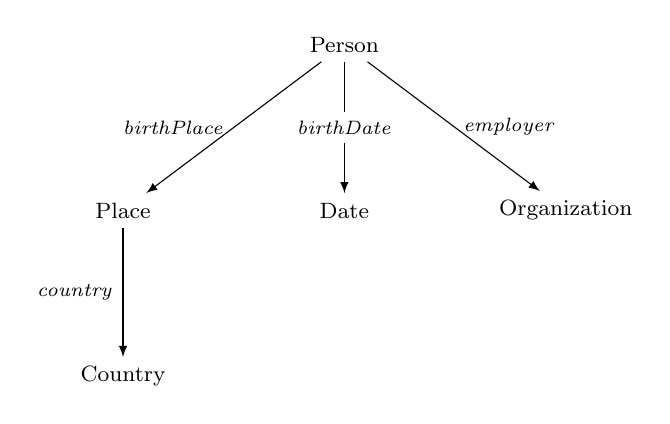
\begin{tikzpicture}[
        sibling distance        = 8em,
        level distance          = 6em,
        edge from parent/.style = {draw, -latex},
        every node/.style       = {font=\footnotesize},
    ]
    \node {Person}
    child {
            node {Place}
            child {
                    node {Country}
                    edge from parent node [left] {\scriptsize{\textit{country}}}
                }
            edge from parent node [left] {\scriptsize{\textit{birthPlace}}}
        }
    child {
            node {Date}
            edge from parent node [fill=white] {\scriptsize{\textit{birthDate}}}
        }
    child {
            node {Organization}
            edge from parent node [right] {\scriptsize{\textit{employer}}}
        };
\end{tikzpicture}
\end{document}